\chapter{Idea of the Program}
\label{cha:program_idea}

The goal of the program is to efficiently plan a path with a given start, end and map, using a genetic algorithm. While not planned as a framework for GA development, the GA parameters and functions still have to be easily adjustable to allow for fast optimization. Both the map and the vehicle need also be configurable so the program can quickly be adapted to a given task. The path optimization algorithm by the AG Echtzeitsysteme is used to obtain a usable path from the generated one in order to make sure the result is not just theoretically a good solution but in fact a drivable path.
The basic idea is a simple GUI based program in which a path can be planned and plotted with the simple click of a button but which also allows modifications to the map, algorithm and vehicle necessary to adapt to any required situation.

\section{Map}
\label{sec:map}

The map has to be given as a simple image (.png) file in which empty areas are white and walls are black. While a different representation of the environment may be better suited for collision detection, this simple map format makes it easier to create new maps for any given area. The map is assumed to be 2 dimensional, so height differences are not considered, and only about 40x20 m in size. The default image size is 1024x512 pixels, other sizes are possible but may lead to problems with the map overlay so any map should be re-sized to this. On start-up, a boolean array of the same size as the map is created and filled with values obtained from the given image, where every white pixel is true and every black pixel is false. This array is used for collision detection while the map itself is only used as a texture background for the GUI.

\section{Vehicle}
\label{sec:vehicle}

The vehicle is saved in a format similar to the one described in \ref{sec:previous_knowledge_vehicle}. For every element of the vehicle the values M and L are saved, which determine the length of the front and rear of the trailer respectively, measured from the axle. In accordance with that representation, the tractive unit is assumed to be 2 parts with a rigid coupling in between. A tractive unit without any trailers is generated randomly every time the program is started, so one can immediately start planning a path without having to configure a vehicle first every time. If a specific vehicle is required, adjustments can be made in the vehicle tab of the GUI. In this tab, M and L can be adjusted for every part of the vehicle, more trailers can be added and vehicles can be saved for later use. While the program can theoretically handle an infinite number of trailers it is currently meant to be used with only one.
For a complete representation of the vehicle more information is required than just the size of every given part, that is, the configuration of the vehicle, found in the configuration tab. This configuration contains the starting point of the vehicle, as well as the angles between all its elements. Effectively, only the angles can be adjusted, the position of the steering vehicle is assumed to be the same as the starting position of the path, set in the main tab, and all other vehicle parts' positions are obtained from that starting position and the elements' angles. The configuration, too, can be saved and loaded.

\section{Path Representation}
\label{sec:path_representation}

To make the representation within the GA easier, certain limitations are enforced on the paths generated by this program, however, most of these are not really constraining since a general-n-trailer is limited in its possible configuration space to begin with. In order to get a fixed genome length we assume every path to be made up of exactly 20 parts. Paths of length 0 are not possible since any given path part has a minimum length of 0.5 meters, similarly, paths longer than 80 meters are not possible but should not be necessary either due to the limitation of the map-size.
A path is represented as a Linked List of path primitives, which can be either a curve or a line. A curve, or CirclePathPart, has an angle, a start angle, an end angle, a radius, a center and a direction, that is, whether it is a left or a right curve. A LinePathPart has a start, end and direction, as well as a speed and a boolean value determining whether the vehicle is driving in reverse or not, however neither of these are used in the current implementation of the program and are simply set to default values. The values of any given path part are either set randomly \ref{sec:generation_0}, obtained from a newly generated genome \ref{cha:algorithm_details} or set by the previous path part, for example, the direction of a LinePathPart can only be the direction of the previous Path Part since no rough edges are permitted.
Due to the selected information encoded in the genome the maximum value of any of these variables as well as the step size between these values are limited. Any given  path part can be between 0.5 and 4 meters long and, in case it is a curve, have an angle between 10° and 45° in steps of 5°. A more detailed path can easily be achieved by extending the length of the genome \ref{sec:genome_representation}, but this would also slow down computation.

\section{Generation 0} % (fold)
\label{sec:generation_0}

The initial generation, also known as generation 0, is obtained by generating random paths and converting these into the genome format, see \ref{sec:genome_representation} for further details on the exact representation. A function generatePath() in the PathPrimitives class is used to randomly generate a path of a fixed length, by default 20 path parts, as well as calculating the corresponding genome. This function generatePath() uses the function getRandomPathPart() of the same class, which generates a path part within the limitations given in \ref{sec:path_representation}.
After enough paths have been obtained, all of them are evaluated.

\section{Evaluation} % (fold)
\label{sec:evaluation}

The evaluation is done using a simple weighted fitness function which considers both the distance from the end of the path to the original goal as well as the number of collisions, leaving the map is also counted towards the collision value. The weight of these two factors can be adjusted but is by default set to 2 to 3 for the goal distance. More factors, like the length of the path, the number of turns or the minimal distance to obstacles could be considered in this function as well, but are currently not implemented. It should be noted that the path evaluated here is not the path obtained from the GA directly, but the generated path after it has gone through the simulation class, which uses the path optimization from AG Echtzeitysteme to transform it into a path drivable by the given vehicle. 

\section{Generation 1+} % (fold)
\label{sec:generation_1+}

Further generations are evaluated in the same way as the initial one, but are obtained by genetic crossing and not randomly. The exact process used in this implementation of the genetic algorithm is described in \ref{cha:algorithm_details}.

\section{GUI}
\label{sec:gui}

The full GUI can be seen in \ref{pic:gui_full_main}. On the left we can see a sample map which can be replaced either in the code or by clicking the "`Load Map"' button on the right and providing a fitting image, see \ref{sec:map}. Black areas on the map are obstacles while white areas are available. The blue dot marks our target destination, the red one our starting point. The lines at the red dot are our current vehicle, the tiny red dot within our vehicle is a coupling, in this case a rigid one since we only have a tractive unit by default. On the right of the map we have buttons for loading a new map, starting the path finding algorithm (Start), starting an entire set of iterations for evaluation purposes (Evaluation), drawing a single random path (Start Path) and obtaining a simulation for a given path (Drive). Next to the "`Drive"' button is a small text box which shows the current generation the algorithm is computing. The current path's genome is shown in the box below those five buttons, every line consists of 8 numbers and represents exactly one path part, as such there are 20 lines. This box is usually read-only, but it can be modified by unchecking the "`Genome Read Only"' box next to it. This way, a previously saved path's genome can be put in and a simulation can be obtained by pressing "`Drive"'. The "`Show Current End"' button shows the configuration of the vehicle at the end of the current path, this could be used in the fitness function but is not yet implemented. The "`Debug Population"' check box causes the algorithm to stop after each generation and output all computed paths along with their rating. 
In \ref{pic:gui_vehicle} we can see the vehicle tab of the GUI which allows us to save, load and modify our general-n-trailer. Each vehicle part is defined by its $M$ and $L$ values, see \ref{sec:previous_knowledge_vehicle}. In the example shown here only the tractive unit, which is generated randomly every time the program is started, is defined, this is the default setting. More trailers can be added by clicking "`Add Box"', filling in the values and then clicking "`Add Axle"'. "`Save"' and "`Load"' will open a dialogue to save the current vehicle to a text file or loading a suitable file. "`Reset"' removes all trailers and goes back to the vehicle that was generated at the beginning.
\ref{pic:gui_configuration} shows the configuration tab which allows the modification of the current vehicle's position and steering angles. The slider bar adjusts the current trailer's angle relative to its predecessor, the trailer to be modified can be chosen in the drop down menu below. Since the default vehicle only has a tractive unit, which has a rigid coupling, there is only one axle available at the beginning, which defines the starting angle. Just like the vehicle, this configuration can be saved, loaded and reset, it should be noted that it is only possible to load a configuration when it fits the current vehicle's number of trailers. Below, the start and end coordinates can bet set, the colours correspond to the points on the map. By selecting "`End Conf"' on the right a target configuration can be set, however, this is not needed at the moment since only the distance to the destination is considered in the fitness function, not the entire configuration.

\begin{figure}[b]
\centering
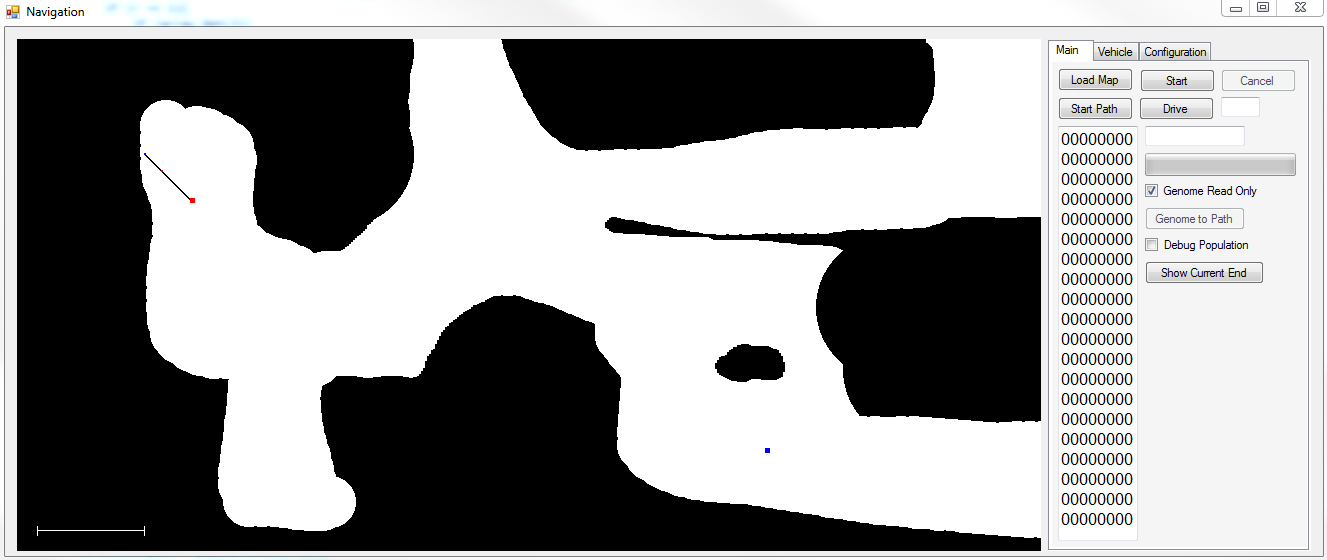
\includegraphics[width=0.75\textwidth]{./Chapters/Figures/gui_full_main.png}
\caption{The full view of the GUI with a sample map on the left and the Main window on the right\label{pic:gui_full_main}}
\end{figure}

\begin{figure}[b]
\centering
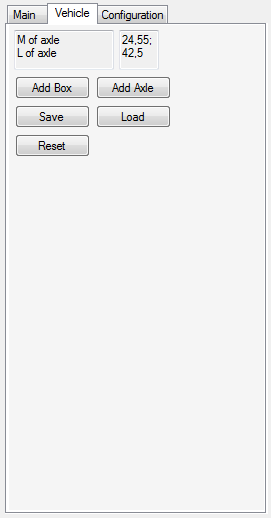
\includegraphics[width=0.75\textwidth]{./Chapters/Figures/gui_vehicle.png}
\caption{The GUIs vehicle Tab\label{pic:gui_vehicle}}
\end{figure}

\begin{figure}[b]
\centering
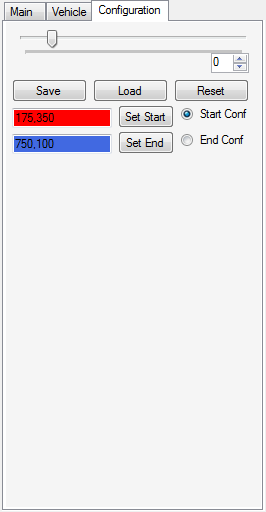
\includegraphics[width=0.75\textwidth]{./Chapters/Figures/gui_configuration.png}
\caption{The GUIs configuration Tab\label{pic:gui_configuration}}
\end{figure}

